\chapter{Capa de lógica}

Este capítulo se ocupa de describir la capa de lógica del sistema, que se encarga de procesar los datos extraídos y exponerlos como recursos accesibles mediante una \gls{API REST}. Primeramente, inicia por justificar la construcción de un API REST como interfaz de la capa de lógica. Posteriormente, se detalla por completo el diseño del API, desde dos perspectivas: por un lado, se describe la estructura de los datos y cómo se representan como objetos, en particular como clases, agnósticas de la fuente de los datos y de la implementación de la API; por otro lado, se expone el diseño de la interfaz del API, detallando los recursos que expone, su representación y los endpoints que brinda para acceder a ellos. Finalmente, se dedica una sección a la calidad del código, detallando las herramientas y prácticas empleadas para garantizar la calidad del código.

\section{¿Por qué un API REST?}

Antes de entrar en detalles sobre el diseño del API, es importante justificar la elección de un API REST como interfaz de la capa de lógica del sistema. En primer lugar, un API REST es una interfaz de programación de aplicaciones que sigue los principios del estilo arquitectónico \gls{REST}. Este estilo se basa en la transferencia de representaciones de recursos, que son identificados por \glslink{URI}{URIs}, y la manipulación de estos recursos mediante métodos estándar de \gls{HTTP}. En particular, un API REST es una interfaz que permite la interoperabilidad de aplicaciones heterogéneas, permitiendo a un programa acceder a las funciones y datos de otro. En el caso de este proyecto, un API REST es la interfaz ideal para exponer los datos procesados por la capa de lógica, ya que permite a cualquier aplicación, como el frontend del perfil del estudiante, acceder a estos datos de manera sencilla y eficiente.

En los últimos años, los API REST han ganado popularidad en el desarrollo de aplicaciones web, ya que son fáciles de entender, escalables y flexibles. Además, un API REST es independiente de la implementación subyacente, lo que significa que el frontend del perfil del estudiante no necesita conocer los detalles de cómo se procesan los datos o cómo se almacenan, sino que solo necesita conocer la interfaz del API. Por último, un API REST es fácil de probar y depurar, ya que se basa en estándares abiertos y bien conocidos, como \gls{HTTP} y \gls{JSON}.

Todo esto hace que un API REST sea la elección ideal para la capa de lógica de este sistema, ya que permite exponer los datos procesados de manera sencilla y eficiente, independiente de la implementación subyacente, y fácil de probar y depurar.

\section{Diseño del API}

El diseño del API se divide en dos partes. La primera parte está en el marco de la programación orientada a objetos, y se encarga de describir cuál es la estructura de clases del API: qué clases existen, cómo se relacionan entre sí y qué atributos tienen. La segunda parte se enfoca en la interfaz del API, es decir, en cómo se exponen los datos procesados como recursos accesibles mediante una API REST. Eso incluye cuáles son los recursos que se exponen, cómo se representan, en qué formato se devuelven al cliente y cuáles son los endpoints que brinda el API para acceder a estos recursos.

Es importante señalar que el diseño del API es completamente independiente de dos factores: por un lado, de la fuente de los datos, es decir, de cómo se extraen los datos de las fuentes originales; por otro lado, de la implementación del API, es decir, de qué lenguaje y cuál framework se utiliza para escribir el código del API. En este sentido, esta sección es independiente del capítulo anterior, que estudia la capa de datos, y de la sección siguiente, que explica la implementación del API.

\subsection{Estructura de clases del API}

Para modelar la información del Perfil del estudiante como objetos se optó por realizar un diagrama de clases conforme al estándar \gls{UML}. Esto tiene la ventaja de que permite visualizar de manera clara y concisa la estructura de clases del API y de que es un artefacto bien conocido y ampliamente utilizado en el desarrollo de software.

\subsubsection{Diagrama de clases}

Se realizaron varias iteraciones en la construcción del diagrama de clases, teniendo en cuenta las necesidades del frontend del perfil del estudiante y las restricciones de la capa de datos. La figura \ref{fig:diagrama_clases} muestra el diagrama de clases final del API.

\begin{figure}[h]
	\centering
	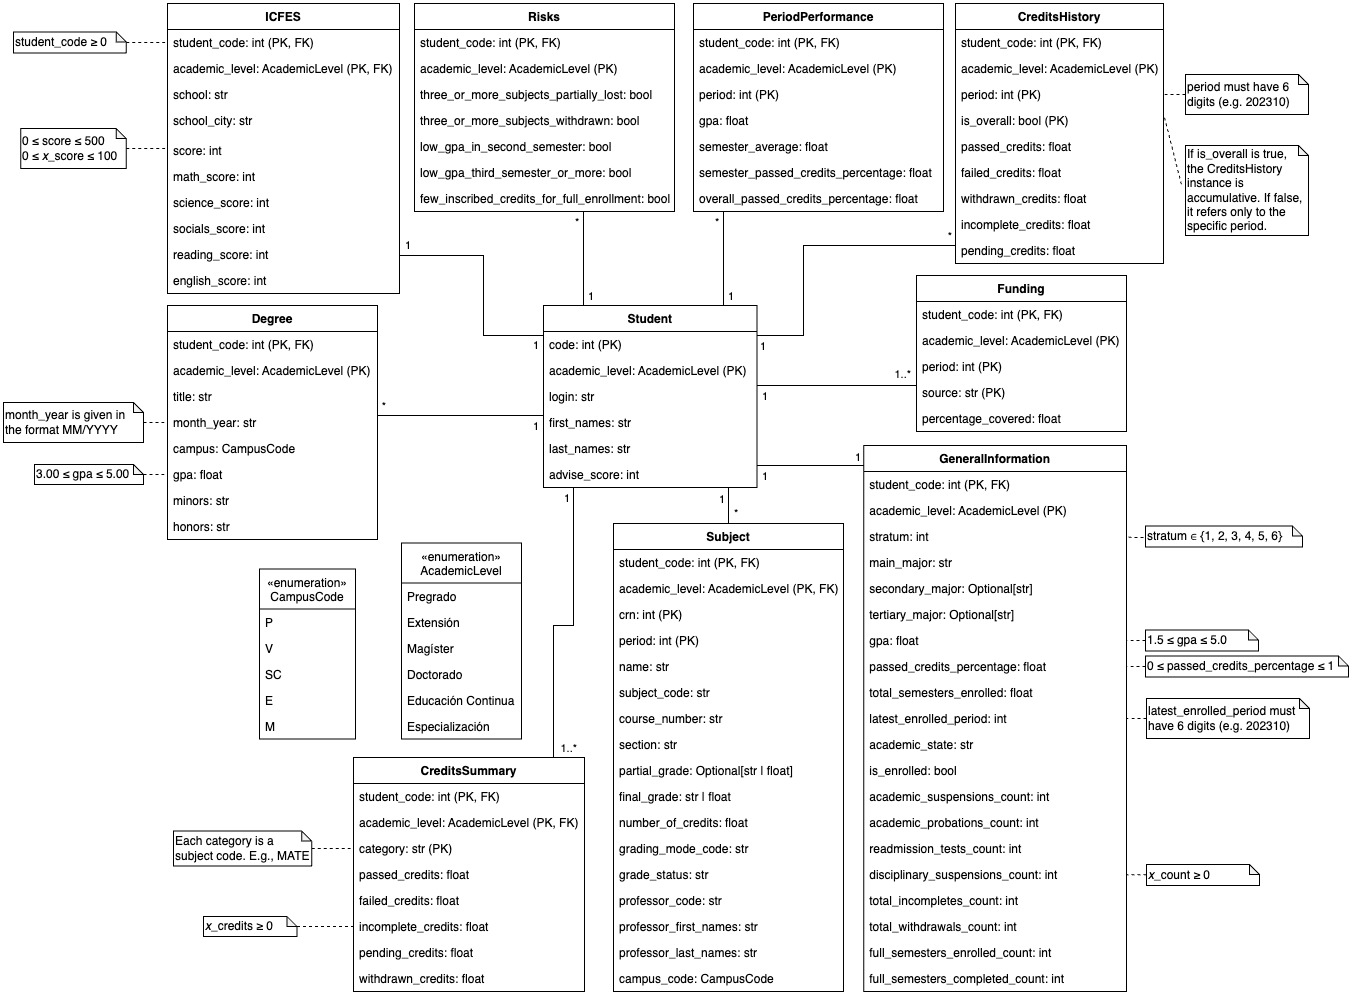
\includegraphics[width=\textwidth]{img/diagrama-clases.jpg}
	\caption{Diagrama de clases del API}
	\label{fig:diagrama_clases}
\end{figure}

El diagrama de clases está escrito en inglés, siguiendo las convenciones de UML. Cada clase tiene un nombre, que es un sustantivo en singular, y una serie de atributos. Los atributos están escritos en el formato \texttt{nombre: tipo}, donde \texttt{nombre} es el nombre del atributo y \texttt{tipo} es el tipo de dato del atributo. Por conveniencia, los tipos de datos empleados son los mismos que se utilizan en el lenguaje de programación Python, que es el lenguaje en el que se implementa el API, pero bien podrían usarse los tipos de datos de cualquier otro lenguaje de programación orientado a objetos sin afectar semánticamente el diagrama de clases, por lo que mantiene su independencia de la implementación.

\subsubsection{Clases del API}

La estructura de clases del API se basa en el principio de responsabilidad única, que establece que cada clase debe tener una sola responsabilidad y representar un solo concepto en el dominio del problema. Las clases propuestas en el diagrama se presentan alfabetizadas en la tabla \ref{tab:clases}, con su nombre original en inglés, la traducción al español y una breve descripción de su responsabilidad.

\begin{longtblr}[
		caption = {Clases del API y sus responsabilidades},
		label = {tab:clases},
	]{
		colspec = {X[1,l] X[1,l] X[2,l]}
	}
	\hline
	\textbf{Nombre original} & \textbf{Nombre traducido}       & \textbf{Responsabilidad}                                                                                                                                                                                                                                                                                             \\
	\hline
	CreditsHistory           & Historial de créditos           & Rastrea el estado global de los créditos del estudiante, incluyendoaprobados, reprobados, retirados, pendientes e incompletos, tanto para periodos específicos, por ejemplo un semestre particular, como en general hasta la fecha.                                                                                  \\
	CreditsSummary           & Resumen de créditos             & Proporciona un desglose categórico de los créditos aprobados, reprobados, retirados, pendientes e incompletos, para una categoría específica de materias. Algunos ejemplos de categoría pueden ser: las materias de la carrera principal, las materias de matemáticas, las materias de física, entre otras.          \\
	Degree                   & Título                          & Almacena información sobre los títulos académicos obtenidos por el estudiante, como el nombre del título, el campus, el promedio y menciones especiales, como títulos con honores.                                                                                                                                   \\
	Funding                  & Financiamiento                  & Detalla las fuentes de financiamiento del estudiante, que pueden incluir becas y créditos educativos, con el porcentaje cubierto por cada fuente.                                                                                                                                                                    \\
	GeneralInformation       & Información general             & Contiene datos generales del estudiante, como su carrera principal, estrato, GPA actual, entre otros indicadores relevantes.                                                                                                                                                                                         \\
	ICFES                    & ICFES                           & Almacena los puntajes del estudiante en las áreas evaluadas por el examen ICFES, como matemáticas, lectura y ciencias.                                                                                                                                                                                               \\
	PeriodPerformance        & Rendimiento por\newline periodo & Guarda información del desempeño académico del estudiante en un periodo específico, incluyendo el promedio del semestre y el porcentaje de créditos aprobados.                                                                                                                                                       \\
	Risks                    & Riesgos                         & Identifica indicadores de riesgo académico, como bajo GPA en los primeros semestres o retiro de múltiples materias.                                                                                                                                                                                                  \\
	Student                  & Estudiante                      & Representa a un estudiante de la universidad cuando se encontraba en un nivel académico específico. Almacena la información esencial para la identificación del estudiante, como nombres, apellidos, código y usuario (\texttt{login}, que corresponde al nombre de usuario en el correo electrónico institucional). \\
	Subject                  & Materia                         & Representa una materia específica cursada por el estudiante, incluyendo el nombre, el código, los créditos, el profesor, la nota obtenida y el estado de la materia.                                                                                                                                                 \\
	\hline
\end{longtblr}

Como complemento del diagrama de clases y de la tabla \ref{tab:clases}, vale la pena ahondar en algunas de las decisiones de diseño que se tomaron en la creación de las clases con base en el dominio del negocio:
\begin{itemize}
	\item La clase \texttt{Student} es la clase principal del modelo. Resalta que no representa a un estudiante por completo, sino que representa a un estudiante en un nivel académico específico. Esto se debe a que resulta conveniente tratar de forma distinta al mismo estudiante en diferentes niveles académicos, ya que su contexto puede haber cambiado significativamente: el título al que aspira es distinto, las materias que cursa son distintas, su desempeño académico puede haber mejorado o empeorado, e incluso su situación socioeconómica puede haber cambiado. La misma persona en pregrado no puede ser tratada de la misma forma que en posgrado.
	\item La clase \texttt{CreditsSummary} es una clase auxiliar que se encarga de proporcionar un desglose categórico de los créditos aprobados, reprobados, retirados, pendientes e incompletos, para una categoría específica de materias. Naturalmente, no para todos los estudiantes se incluyen las mismas categorías. Es decir, para un estudiante de ingeniería, Categorías relevantes pueden ser las materias Específicas de su rama del ingeniería, las materias de matemática y las materias de física. Sin embargo, para un estudiante de arte, incluso si el estudiante ha optado por cursar materias de matemática y física, esas categorías pueden no ser relevantes para su desempeño académico. Esto es un matiz que es difícil representar en un diagrama de clases y que corresponde a especificidades del dominio del problema, por lo cual se aclara en este apartado.
	\item Puede que el lector se haya percatado que la clase \texttt{Risks} está nombrada con un sustantivo en plural, lo cual aparentemente transgrede las convenciones de construcción de diagramas de clase. Eso no es un error, sino una decisión consciente de diseño. Se debe a que la clase \texttt{Risks} no representa un riesgo académico en particular, sino que cada instancia de la clase corresponde a un conjunto de riesgos académicos, entre ellos bajo GPA y retiro de múltiples materias. Por lo tanto, el nombre en plural es más adecuado para representar la naturaleza de la clase.
\end{itemize}

\subsubsection{Relaciones entre las clases}

Las relaciones entre las clases se representan mediante líneas que unen las clases. Las relaciones en este diagrama son muy simples, lo cual fue una elección deliberada en pos de la simplicidad y la claridad. Cada línea representa una asociación entre dos clases y en sus extremos cuenta con números que indican la multiplicidad de la asociación, es decir, cuántos objetos de una clase están asociados con cuántos objetos de la otra clase. Un asterisco indica que hay muchos objetos asociados, mientras que un número indica la cantidad exacta de objetos asociados. Por ejemplo, un estudiante está asociado con muchas materias, pero cada materia está asociada con un solo estudiante, por lo que la asociación entre la clase \texttt{Student} y la clase \texttt{Subject} es de uno a muchos, representada por la línea que une ambas clases con un 1 en el extremo de la clase \texttt{Student} y un asterisco en el extremo de la clase \texttt{Subject}. La tabla \ref{tab:relaciones} detalla las relaciones entre las clases del diagrama de clases, con una breve descripción de la relación y la multiplicidad de la asociación. Se ordenan en orden de aparición, de arriba a abajo y de izquierda a derecha, en el diagrama de clases.


\begin{longtblr}[
		caption = {Relaciones entre las clases del diagrama de clases},
		label = {tab:relaciones},
	]{
		colspec = {X[1,l] X[2,l] X[3,l]}
	}

	\hline
	\textbf{Clase 1} & \textbf{Clase 2}            & \textbf{Descripción y Multiplicidad}                                                                                                                         \\  \hline
	\texttt{Student} & \texttt{GeneralInformation} & Un estudiante está asociado con una única instancia de información general. Multiplicidad: 1 a 1.                                                            \\
	\texttt{Student} & \texttt{ICFES}              & Un estudiante puede tener una única instancia de resultados del ICFES. Multiplicidad: 1 a 1.                                                                 \\
	\texttt{Student} & \texttt{Risks}              & Un estudiante tiene una única instancia de indicadores de riesgos académicos. Multiplicidad: 1 a 1.                                                          \\
	\texttt{Student} & \texttt{PeriodPerformance}  & Un estudiante puede estar asociado con muchos periodos de desempeño académico. Multiplicidad: 1 a muchos.                                                    \\
	\texttt{Student} & \texttt{CreditsHistory}     & Un estudiante puede tener muchos historiales de créditos, cada uno relacionado con un periodo específico o de manera acumulativa. Multiplicidad: 1 a muchos. \\
	\texttt{Student} & \texttt{CreditsSummary}     & Un estudiante tiene un resumen de créditos categorizado. Multiplicidad: 1 a 1.                                                                               \\
	\texttt{Student} & \texttt{Subject}            & Un estudiante está asociado con muchas materias, pero cada materia pertenece a un único estudiante. Multiplicidad: 1 a muchos.                               \\
	\texttt{Student} & \texttt{Degrees}            & Un estudiante puede haber obtenido múltiples títulos. Multiplicidad: 1 a muchos.                                                                             \\
	\texttt{Student} & \texttt{Funding}            & Un estudiante puede tener múltiples fuentes de financiamiento. Multiplicidad: 1 a muchos.                                                                    \\
	\texttt{Subject} & \texttt{CreditsSummary}     & Cada materia está categorizada en un resumen de créditos. Multiplicidad: 1 a 1.
	\\
	\hline
\end{longtblr}

\subsubsection{Reglas de negocio en el diagrama de clases}

En el diagrama de clases se pueden evidenciar anotaciones en algunos atributos. Varias de estas anotaciones corresponden a restricciones de integridad que se deben cumplir en el modelo de datos, que en últimas representan reglas del dominio del problema. A esto, usualmente se le denomina \textit{reglas de negocio} y son restricciones que se deben cumplir en el modelo de datos para que reflejen la realidad de manera fiel.

La tabla \ref{tab:anotaciones} detalla las anotaciones en el diagrama de clases que tienen esa función, junto con su significado en términos del dominio del problema, es decir, en el contexto de la Universidad. Se ordenan en orden de aparición en el diagrama de clases, de arriba a abajo y de izquierda a derecha.

\begin{longtblr}[
		caption = {Anotaciones del diagrama de clases y su significado},
		label = {tab:anotaciones},
	]{
		colspec = {X[1,l] X[2,l] X[2,l]},
	}
	\hline
	\textbf{Anotación}                                                           & \textbf{Significado}                                                                                                       & \textbf{Justificación}                                                                                                                                                                                                                                             \\
	\hline
	\texttt{student\_code \ensuremath{\geq} 0}                                   & El código del estudiante debe ser mayor o igual a 0                                                                        & El código del estudiante debe ser un entero positivo que identifica únicamente a cada estudiante. No se permiten códigos negativos.                                                                                                                                \\
	\texttt{0 \ensuremath{\leq} score \ensuremath{\leq} 500}                     & El puntaje del ICFES (formalmente, la prueba Saber 11) debe estar entre 0 y 500                                            & El puntaje máximo en la prueba Saber 11 es 500, y el mínimo es 0.                                                                                                                                                                                                  \\
	\texttt{0 \ensuremath{\leq} x\_score \ensuremath{\leq} 100}                  & Los puntajes de las áreas evaluadas por el ICFES deben estar entre 0 y 100                                                 & Los puntajes de las áreas evaluadas por el ICFES se normalizan a una escala de 0 a 100.                                                                                                                                                                            \\
	\texttt{month\_year is given in the format MM/YYYY}                          & La fecha de graduación, que se representa como un mes y un año, debe tener el formato MM/YYYY                              & La fecha de graduación se codifica en el formato de mes y año para garantizar consistencia en los registros.                                                                                                                                                       \\
	\texttt{3.00 \ensuremath{\leq} gpa \ensuremath{\leq} 5.0}                    & El GPA debe estar entre 3.0 y 5.0                                                                                          & En el sistema de la Universidad, el GPA mínimo para graduarse es 3.0, y el máximo posible es 5.0.                                                                                                                                                                  \\
	\texttt{Each category is a subject code. E.g., MATE}                         & Cada categoría de un Resumen de créditos es un código de materia. Por ejemplo, MATE representa las materias de matemáticas & Las categorías de un Resumen de créditos se representan con códigos de materia. Esta decisión de diseño se explica en detalle arriba, en la descripción de la clase \texttt{CreditsSummary}.                                                                       \\
	\texttt{x\_credits \ensuremath{\geq} 0}                                      & Los créditos aprobados, reprobados, retirados, pendientes e incompletos deben ser mayores o iguales a 0                    & No tiene sentido registrar un número negativo de créditos en ningún contexto académico.                                                                                                                                                                            \\
	\texttt{period must have 6 digits (e.g. 202310)}                             & El periodo académico debe tener 6 dígitos                                                                                  & Los periodos académicos se codifican en el formato de año seguido por el indicador del tipo de periodo. Usualmente se usa un guión entre el año y el tipo de periodo, e.g., 2023-10, pero en este caso resulta más conveniente usar un número entero de 6 dígitos. \\
	\texttt{stratum \ensuremath{\in} \{1, 2, 3, 4, 5, 6\}}                       & El estrato socioeconómico debe estar entre 1 y 6                                                                           & Los estratos socioeconómicos en Colombia están normados en este rango por ley. Si el estudiante no es residente en Colombia, no se registra su estrato.                                                                                                            \\
	\texttt{1.5 \ensuremath{\leq} gpa \ensuremath{\leq} 5.0}                     & El GPA debe estar entre 1.5 y 5.0                                                                                          & En el sistema de la Universidad, el GPA mínimo posible es 1.5, y el máximo posible es 5.0.                                                                                                                                                                         \\
	\texttt{0 \ensuremath{\leq} passed\_credits\_percentage \ensuremath{\leq} 1} & El porcentaje de créditos aprobados debe estar entre 0 y 1                                                                 & Todo porcentaje es un número entre 0 y 1, inclusive.                                                                                                                                                                                                               \\
	\texttt{latest\_enrolled\_period must have 6 digits (e.g. 202310)}           & El periodo académico más reciente en el que el estudiante estuvo inscrito debe tener 6 dígitos                             & Esta explicación es análoga a la de la anotación \texttt{period must have 6 digits (e.g. 202310)}.                                                                                                                                                                 \\
	\hline
\end{longtblr}

\subsection{Diseño de la interfaz del API}

% TODO: Acá va qué recursos son, la representación, el formato, los endpoints, etc.

\section{Implementación del API}

\section{Calidad de código}

%TODO: Agradecimiento a Ruby y a Cardozo, la primera mi profesora en Métricas y Calidad de SW; el segundo además profesor mío en Reinforcement Learning

Teniendo en cuenta que el software producido es de alto valor para la universidad y por ende probablemente querrá ser mantenido, extendido y reutilizado en el futuro, su desarrollo fue sometido a rigurosos estándares de calidad de código. Esta sección detalla las herramientas y prácticas empleadas para garantizar la calidad del código.

\begin{resumen}
	Se realizaron múltiples esfuerzos para garantizar la calidad del código del proyecto:
	\begin{itemize}
		\item Se documentaron todas las funciones y métodos con \glslink{docstring}{docstrings} siguiendo la convención de \gls{Pandas}.
		\item Se utilizaron \gls{isort} y \gls{black} como \glslink{formateador}{formateadores}, \gls{Flake8} y \gls{SonarLint} como \glslink{linter}{linters}, y \gls{doctest} y \gls{Pytest} para las \gls{pruebas unitarias}.
		\item Se configuró un \gls{hook} de pre-commit de \gls{Git} para garantizar el formato y ejecutar las pruebas antes de cada commit.
		\item Se estableció un \gls{pipeline} en \gls{GitHub Actions} que ejecuta las pruebas, genera un reporte de cobertura y lo envía a \gls{SonarQube}.
		\item Se configuró \gls{SonarQube} para realizar análisis estático sobre el código, usando el \gls{perfil de calidad} estándar para \gls{Python} 3.11.
	\end{itemize}
\end{resumen}

%TODO: Organizar todo esto para explicar las configuraciones de cada cosa que usé

Todas las funciones y métodos de la \gls{API} están documentados mediante \glslink{docstring}{\textit{docstrings}}. Naturalmente, los docstrings siguen las convenciones definidas en el estándar \href{https://peps.python.org/pep-0257/}{\gls{PEP} 257}. Más aún, debido a que las disposiciones del estándar son notablemente flexibles, se optó por seguir la afamada convención de docstrings de \gls{NumPy}. Más específicamente, se satisfacen todos los lineamientos de la \href{https://python-sprints.github.io/pandas/guide/pandas_docstring.html}{guía de docstrings de \gls{Pandas}}.



Su sintaxis satisface el estilo \glslink{reST}{reStructuredText (REST)},
% TODO: lo cual permite que los docstrings sean procesados por herramientas como \gls{Sphinx}, que genera documentación automáticamente a partir de ellos.



Se hace uso del linter \gls{Flake8},

Se emplea la librería \verb|flake8-docstrings|, con la configuración \verb|docstring-convention=numpy| en el archivo de configuración de Flake8, para verificar que los docstrings sigan la convención de NumPy.



\subsection{Representación de los datos como recursos de una API REST}

Una vez los datos han sido procesados y almacenados en el Blob Storage, se exponen como recursos accesibles mediante una \gls{API REST}. La \gls{API} se encuentra escrita en Python, utilizando el framework FastAPI, y se despliega en un contenedor Docker que reside en una máquina virtual provista por la universidad.

La siguiente sección trata en detalle todos los aspectos técnicos relacionados con este \gls{API REST}. Por lo pronto, basta con mostrar, a alto nivel, cuáles son los recursos que provee la \gls{API} para el consumo por parte del frontend del perfil del estudiante. La tabla \ref{tab:recursos} detalla dichos recursos y la información que contienen. Nótese que el \gls{API} expone muchos más recursos que los mostrados en la tabla, pero solo esos se utilizan en el perfil del estudiante.

\begin{table}[h]
	\centering
	\caption{Recursos de la \gls{API REST}}
	\alternatecolors
	\begin{longtable}{p{3cm}p{8cm}}
		\hline
		\textbf{Ruta del recurso}                     & \textbf{Información}                                                                                                       \\
		\hline
		\verb*|/nes/student/<usuario del estudiante>| & Información básica del estudiante: nombres, apellidos, código, usuario y niveles académicos en los que ha estado inscrito. \\
		% TODO: Completar
		\hline
	\end{longtable}
	\label{tab:recursos}
\end{table}